%File: formatting-instruction.tex
\documentclass[letterpaper]{article}
\usepackage{aaai}
\usepackage{times}
\usepackage{helvet}
\usepackage{courier}
\usepackage{graphicx}
\usepackage{subfigure}
\frenchspacing
\setlength{\pdfpagewidth}{8.5in}
\setlength{\pdfpageheight}{11in}
\usepackage{amsmath}
\pdfinfo{
/Title ( Error Classification in OCR Historic Newspaper Archive using SVM\textsuperscript{multiclass})
/Author (Megha Gupta, Dr. Haimonti Dutta)}
\setcounter{secnumdepth}{1}  
 \begin{document}
% The file aaai.sty is the style file for AAAI Press 
% proceedings, working notes, and technical reports.
%
%\title{Crowdsourced OCR Error Correction Classification using Multi-Class Support Vector Machines}
%\title{Classification of Text Corrected by the Crowd using Support Vector Machines}
\title{CCTC: \textbf{C}lassification of \textbf{C}rowdsourced \textbf{T}ext \textbf{C}orrection}
%\author{Megha Gupta\\Department of Computer Science,\\ IIIT-Delhi, India \\ meghag@iiitd.ac.in 
%\And Dr. Haimonti Dutta\\
%Center for Computational Learning Systems,\\ Columbia University, New York\\ haimonti@iiitd.ac.in}

\author{Haimonti Dutta\thanks{The author is also a visiting assistant professor at IIIT-Delhi.}\\
Center for Computational Learning Systems, \\
Columbia University, \\
New York, NY 10115\\
haimonti@ccls.columbia.edu\\
\And
Megha Gupta \\ 
IIIT-Delhi, India. \\
meghag@iiitd.ac.in
\And 
Brian Geiger \\
University of California, Riverside \\
brian.geiger@ucr.edu
}

\maketitle
\begin{abstract}
\begin{quote}
\noindent Optical Character Recognition (OCR) is a commonly used method of digitizing printed texts so that they can be searched and displayed online, stored compactly and used in text mining applications.\\
The text generated from OCR devices, however, is often garbled due to variations in quality of the input paper, size and style of the font and column layout. This adversely affects retrieval effectiveness; hence the techniques for cleaning the OCR need to be improvised. Often such techniques involve laborious and time consuming manual processing of data.\\
This paper shows the need to devise an algorithm that is scalable for a large dataset. The current state of the art algorithm used for performing multi class classification is not yet scalable. The current algorithm takes a long time to converge in a particular parameter setting.

\end{quote}
\end{abstract}

\section{Introduction}
\label{sec:intro}

Crowdsourcing is used extensively in cultural heritage and digital history related projects in recent years to 
digitize, create and process content and provide editorial or processing interventions. For example, the Australian Newspapers Digitization Program \cite{ADNP} enables communities to explore their rich newspaper heritage by enabling free online public access to over 830,000 newspaper pages containing 8.4 million articles. The public enhanced the data by correcting over 7 million lines of text and adding 200,000 tags and 4600 comments \cite{holley_09}. Picture Australia \cite{pictAus} harvests digital images from other heritage institutions and encourages the public to upload their own images and tag them. FamilySearch \cite{famSearch} made available handwritten digital images of births, deaths and marriage records for transcription by the public. The New York Public Library has 1,277,616 dishes transcribed to date from 17,079 menus. Galaxy Zoo \cite{galZoo} is an online collaborative astronomy project in which users are invited to classify millions of galaxies from digital photos. 

In all of the above crowdsourcing projects, large volumes of data are generated by users. These include tags, folksonomies, flagged content, information on history, relationship and preference data, structured labels describing objects and creative responses \cite{Ridge_11}. In most citizen science projects, however, little statistical analysis is done on the user generated content. Thus assessment of data quality obtained by leveraging the ``wisdom of the crowd" remains an open problem. 

%Before this question can be answered, statistical analysis of the data generated is imperative.

In this paper, we focus on understanding the nature of text corrections done by users of an old historic newspaper archive. The newspapers are made available for searching on the Internet after the following processes take place: (1) the microfilm copy or paper original is scanned; (2) master and Web image files are generated; (3) metadata is assigned for each page to improve the search capability of the newspaper; (4) OCR software is run over high resolution images to create searchable full text and (5) OCR text, images, and metadata are imported into a digital library software program. The OCR scanning process is far from perfect and the documents generated from it contains a large amount of garbled text. A user is presented with a high resolution image of a newspaper page along with erroneous or distorted text from the OCR and is expected to rectify the garbled words as appropriate. A prototype for a system that can be used for \textbf{C}lassification of \textbf{C}rowdsourced \textbf{T}ext \textbf{C}orrection (CCTC) is presented which can answer simple questions such as ``What are the different kinds corrections proposed by users?" and statistics generated from the correction process. 
The output from the system can be used to enhance search and retrieval on the archive.

Our study used log files generated from text correction software in use at the California Digital Newspaper Collection (CDNC)\footnote{http://cdnc.ucr.edu/cgi-bin/cdnc}, which contains over 400,000 pages of newspapers published in California between 1846-1922. 
%To date, the archive has approximately 1680 registered users who have corrected close to 2 million lines of text. 
%The corrections are primarily categorized as changes in spellings, punctuation rectification, addition of content or capitalization. A semi-automatic engine for classifying corrections based on support vector machines is designed.  
To the best of our knowledge, this is the first attempt to statistically analyze and model OCR error corrections provided by the crowd. We posit that such a classification system will be beneficial when attempting to compensate the annotators; it can also be used for task allocation if some users are more comfortable with certain type of corrections than others.

%In a bid to serve its patrons better, the CDNC crowdsourced the cleaning of OCR text. To date..

[CHECK THIS] \noindent \textbf{Organization}: Section~\ref{arch} describes the architecture of the proposed system. Section~\ref{sec:data} describes the data obtained from crowd sourcing and pre-processing steps; Section~\ref{sec:methodology} presents the design of the semi-automatic error correction classifier and Section~\ref{sec:evaluation} presents empirical and scalability results using real-world data collected at CDNC. Section~\ref{sec:related} discusses related work in OCR text correction with particular emphasis on systems requiring human intervention. Finally, Section~\ref{sec:conc} concludes the paper.



%The \textit{California Digital Newspaper Collection}\footnote{http://cdnc.ucr.edu/cgi-bin/cdnc} is an initiative of the Center for Bibliographical Studies and Research (CBSR) which is supported in part by the U.S. Institute of Museum and Library Services. It is also supported by the National Endowment for the Humanities (NEH) to digitise California newspapers for the National Digital Newspaper Program (NDNP). It contains over 400,000 pages of significant historical California newspapers published from 1846-1922.\\
%OCR devices are widely used in electronic conversion of scanned images which are handwritten or printed text into a machine encoded text. It finds most successful applications in the field of machine Learning, Artificial Intelligence and Pattern recognition. It deals with the problem of recognising optically generated characters be it offline or online. The performance directly depends on the quality of input document. The more constrained the input is the better will be the performance of the system. But when it comes to unconstrained handwriting, the performance is far from satisfactory. The main application areas for \cite{OCR} like Automatic number plate readers, form readers, signature verification.\\
%This project deals with printed text in the form of Historical Newspaper Articles in the holdings of \cite{cdnc}. One such newspaper, The Amador Ledger published in the early 1900s by the Amador Publishing Company appealed to the community's interests by covering issues unique to gold mining. Patrons of the \cite{cdnc} continue to be interested in studying about the status of the local mining industry and consequently read the Amador Ledger on a regular basis even to this day and correct \cite{OCR} errors as they come across them.\\
%In this paper, we perform error classification using Joachims multi-class Support Vector Machine algorithm called \textit{SVM\textsuperscript{multiclass}}\footnote{http://www.cs.cornell.edu/people/tj/svm\_light/svm\_multiclass.html}. We chose this algorithm as its the state of the art algorithm till now. But the experiments give altogether a different view on this algorithm. This algorithm do not converge quickly on certain parameters which are shown in table ~\ref{table: runtime}


%\begin{figure*}[t]
%\centering
%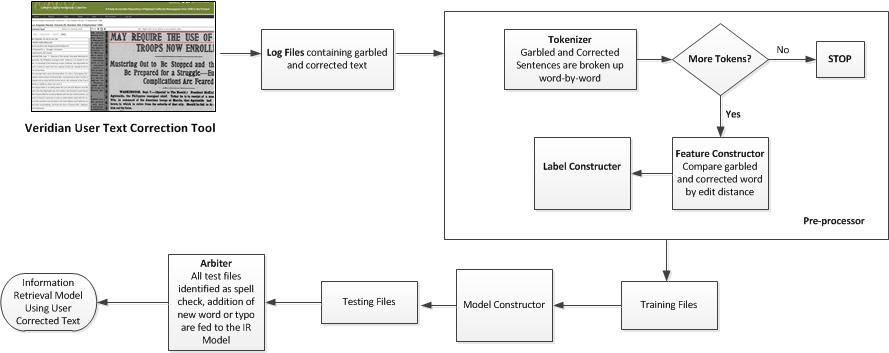
\includegraphics[width=0.8\textheight]{./image/archOCR.jpg}
%\caption{The Architecture of the Proposed System}
%\label{fig:arch}
%\end{figure*}


\section{Architecture of the Proposed System}
\label{arch}


The \textbf{C}lassification of \textbf{C}rowdsourced \textbf{T}ext \textbf{C}orrection (CCTC) system has the following components:

\begin{figure*}[h]
\begin{center}
%\mbox{
\subfigure[Scanned newspaper ``The Amador Ledger" highlighting an article to be corrected by a user.]
{
%%\includegraphics[width=0.6\columnwidth]{odds_20070813_160000rb_M.pdf}
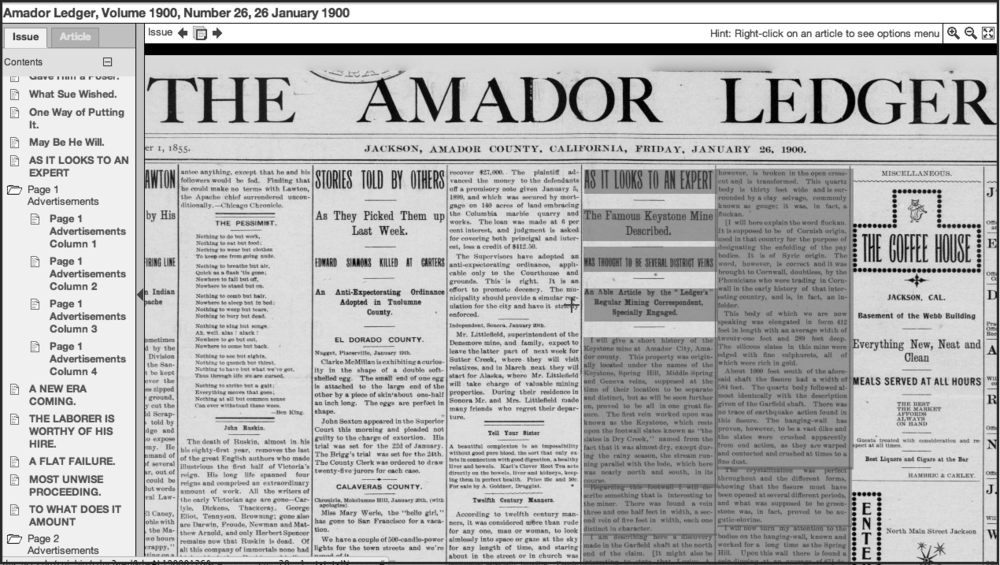
\includegraphics[width=0.48\textwidth]{./image/issue_greyscale.jpg}
\label{fig:T1}
}
\subfigure[The tool used by patrons to annotate articles.]
{
%%\includegraphics[width=0.8\columnwidth]{20070813-C1-7d-roc.pdf}
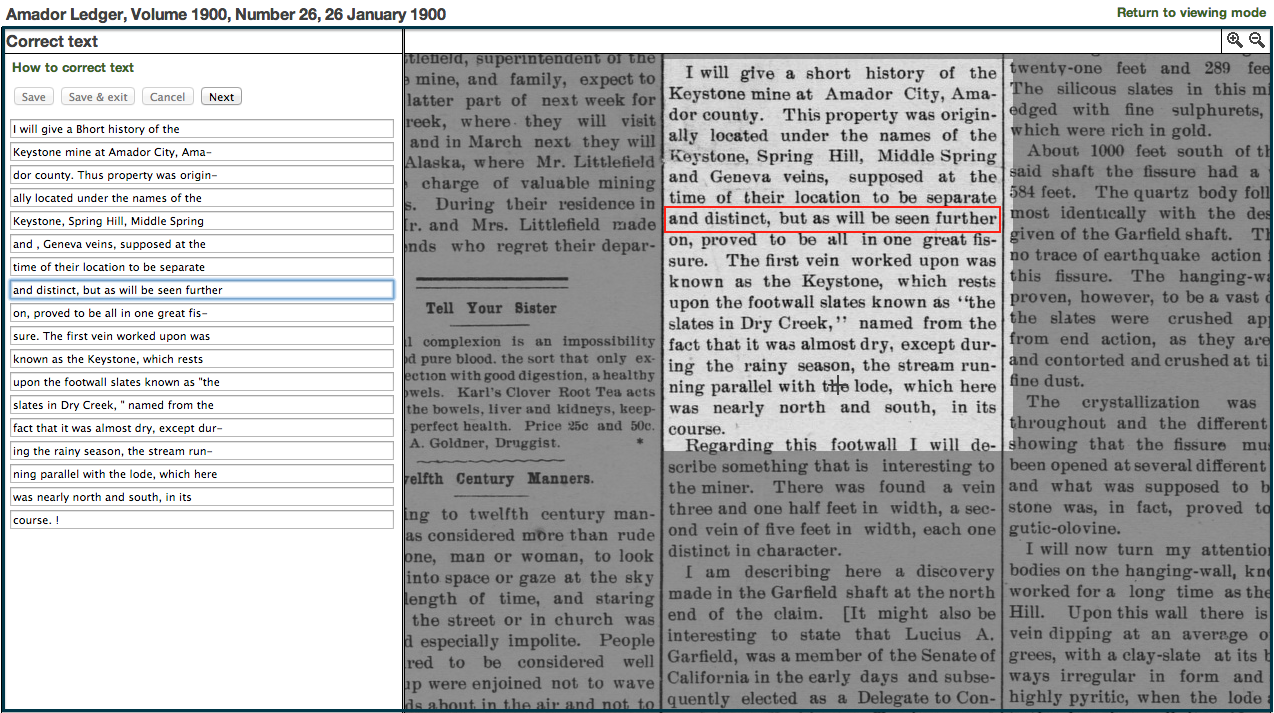
\includegraphics[width=0.48\textwidth]{./image/correction.jpg}
\label{fig:T2}
}
%\caption{Something.}
\label{News_01}
\end{center}
\end{figure*}

\begin{enumerate}


\item The \textbf{Veridian User Text Correction}\footnote{http://veridiansoftware.com/crowdsourcing/} tool which takes as input a scanned page of the newspaper and enables users to correct OCR errors as they come across them.
Figure~\ref{fig:T1} shows an example of a scanned page from ``The Amador Ledger" published on January 26, 1900. The article to be corrected by a user is highlighted. The raw OCR text from the article and the tool used by patrons to correct text is shown in figure ~\ref{fig:T2}.

\item \textbf{Log Files: }All corrections performed by the annotators are recorded in log files. To date approximately 1,705,149 lines have been edited by 848 annotators which resulted in 235 log files. A sample of 191 files have been chosen for our work in this project. Each log file is generated at the issue-level and contains XML data about the pages in the issue. Table~\ref{table:logfile} describes the structure of the log file. The following information is provided about the corrections made by the patrons:
\begin{enumerate}
\item \textit{Page Id: } The id of the page in which editing was done.
\item \textit{Block Id: } The id of the paragraph containing the line corrected by the user.
\item \textit{Line Id: }The id of the line edited by the user.
\item \textit{Old Text Value} is the garbled text generated by the OCR device and replaced by the user.
\item \textit{New Text Value} is the corrected text with which the old text was replaced.
\end{enumerate}

\begin{table}[h]
\begin{center}
\begin{tabular}{l}
\textless TextCorrectedLine lineID="P2\_TL00800"\textgreater \\
\textless OldTextValue\textgreater \textbf{Spll, Stales}\textless /OldTextValue\textgreater \\
\textless NewTextValue\textgreater \textbf{Union Stables}\textless /NewTextValue\textgreater \\
\textless /TextCorrectedLine\textgreater \\
\textless TextCorrectedLine lineID="P2\_TL00801"\textgreater \\
\textless OldTextValue\textgreater \textbf{**?�** Under Webb Hall *}\textless/OldTextValue\textgreater \\
\textless NewTextValue\textgreater \textbf{Under Webb Hall} \textless/NewTextValue\textgreater \\
\textless /TextCorrectedLine\textgreater \\
\end{tabular}
\end{center}
\caption{A segment of the log file}
\label{table:logfile}
\end{table}

\item \textbf{Preprocessor: } The preprocessor has three main components:
\begin{itemize}
\item \textbf{Tokenizer: } The old text and the corresponding new text from the log file is tokenized by white-spaces. There are 44,022 tokens of which 20,137 are corrected by the annotators.

\item \textbf{Feature Constructor: } Features are crafted by computing the Levenshtein edit distance between the old word and its correction. The Levenshtein edit distance \cite{Wagner_74} is defined as the minimum number of single edit operations (insertions, deletions and substitutions) required to convert one string into another. Six binary features are generated as follows: 


\begin{enumerate}
\item \textit{Same Length} : 1, if both the old word and new word have same length and $0$ otherwise. For example, the feature is 1 for the tokens ``Spll," and ``Union" as  both the tokens have same number of characters.
\item \textit{Edit Distance Zero}:  1, if both the words are exactly same and $0$ otherwise. For example, the feature is 1 for tokens ``Under" and ``Under". 
\item \textit{Edit Distance Above One}: 1, if more than one edit operation is required to convert old word to new word and $0$ otherwise. For ``Spll," and ``Union", value is 1 as more than one edit operation is required to convert from old to new token.
\item \textit{Edit Distance Below Three}: 1, if less than three edit operations are required to convert old word to new word and $0$ otherwise. For ``Stales" and ``Stables", value is 1 as less than three edit operations are required to convert from old to new token. 
\item \textit{Edit Distance is 1 and Case Change}: 1, if the two words have edit distance is exactly 1 and the first character of one string change from upper case to lower case or vice versa. For ``Stales" and ``Stables", the value is 0 as there are two conditions to be met. One, when both the tokens have edit distance exactly 1 and second, when there is a upper to lower or lower to upper case change in the first character. Here, the edit distance is exactly 1 but there is no case change.
\item \textit{Punctuation Difference}: 1, if both the old text and new text differ in any of the following punctuation marks (!"\#\$\%\&'*+,-./:;\textless=\textgreater?@[$\backslash$]\^\_`\{\textbar\}\textasciitilde)
. For ``Spll," and ``Union", the value is 1 as the old and new text differ in one of the following punctuation marks
\end{enumerate}

%\begin{figure*}[t]
%\centering
%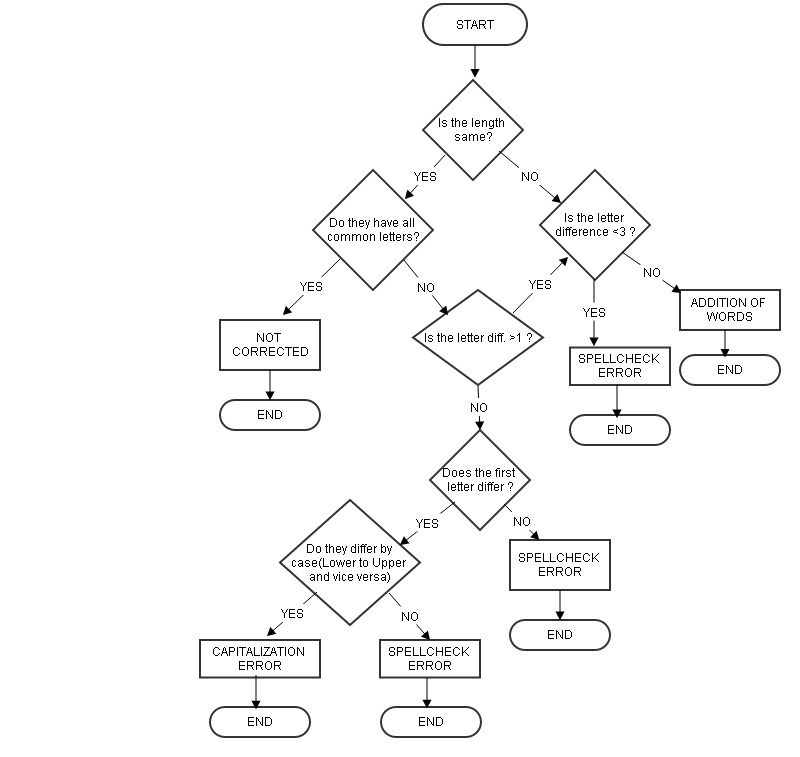
\includegraphics[width=0.9\textwidth]{./image/flowchartnew.jpg}
%%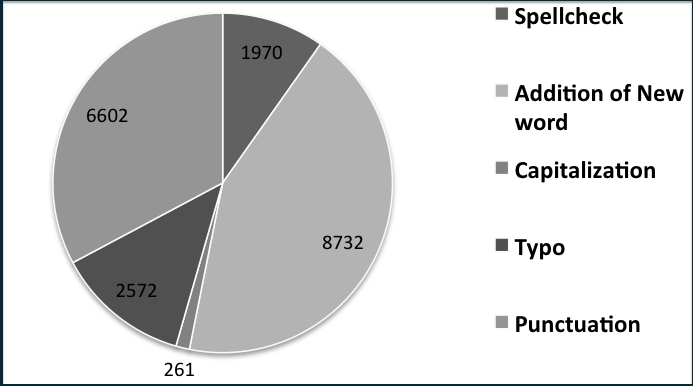
\includegraphics[width=6cm,height=4cm]{./image/error.jpg}
%\caption{Flowchart demonstrating how the labels are generated.}
%\label{fig:flowchart}
%\end{figure*}

\item \textbf{Label Constructor: }The errors rectified by the users are categorized as Spellcheck Error, Addition of a new word, Capitalization Error, Typo and Punctuation error. The logic used in generation of the features can be summarized by the flowchart depicted in Figure~\ref{fig:flowchart}. Specifically,
\begin{enumerate}
\item \textit{Class 1-Spellcheck error: }When the edit distance is between 1 and 3. For example, ``mounten" and ``mountain".
\item \textit{Class 2-Addition of a new word: }When the edit distance is more than 3. For example, ``at" and ``attend".
\item \textit{Class 3-Capitalization error: } When the edit distance of two strings is exactly 1 and first letter of both the strings changes from upper to lower case or vice versa. For example, ``largest" and ``Largest".
\item \textit{Class 4-Typo: } When the edit distance is exactly one and case change is 0. For example, ``teh" and ``the"
\item \textit{Class 5-Punctuation error: }When the two strings differ by special characters contained in the set (!"\#\$\%\&'()*+,-./:;\textless=\textgreater?@[$\backslash$]\^\_`\{\textbar\}\textasciitilde). For example, ``residents" and residents
\item \textit{Class 6-No correction: }When the old and new text are same. For example, plant and plant
\end{enumerate}

The distribution of the these classes in the dataset is shown in Table~\ref{table: classes}.

\begin{table}[htdp]
\begin{center}
\begin{tabular}{| c | c |}
\hline
 Class  & No. of Instances \\
\hline
 Spellcheck & 1970 \\
%\hline 
 Addition of new word & 8732 \\
%\hline
 Capitalization & 261 \\
%\hline
Typo & 2572 \\
%\hline
Punctuation & 6602 \\
%\hline
No correction & 23885 \\
\hline
Total & 44022 \\
\hline
\end{tabular}
\end{center}
\caption{Class Distribution}
\label{table: classes}
\end{table}

\end{itemize}
%\begin{figure}[h]
%\centering
%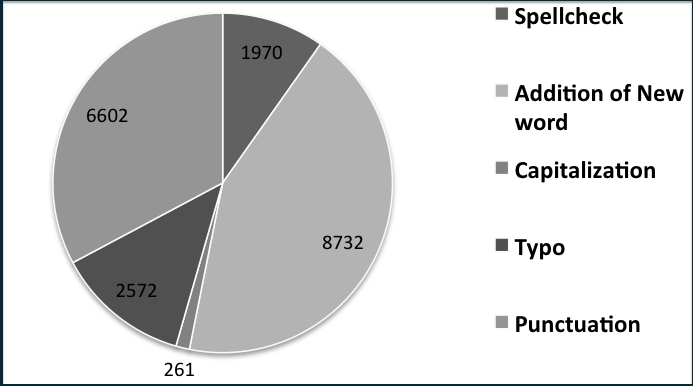
\includegraphics[width=0.48\textwidth]{./image/error.jpg}
%%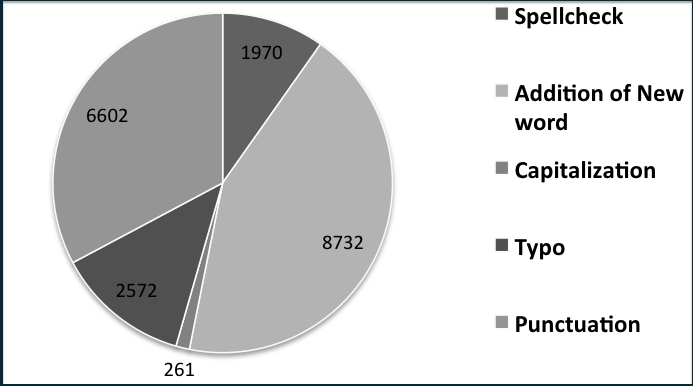
\includegraphics[width=6cm,height=4cm]{./image/error.jpg}
%\caption{Error Classification}
%\label{fig:stats}
%\end{figure}


%The error classes were restricted to 6 classes including Spellcheck Error, Addition of a new word, Capitalization Error, Typo, Punctuation Error and No correction



%The dataset was parsed to a format used by the Joachim's multi class SVM algorithm which is represented as\\
%\textless target\textgreater\space\textless feature\textgreater:\textless value\textgreater ......\textless feature\textgreater:\textless value\textgreater\\
%The number of rows in the dataset is 44,022. 
%The class distribution in the dataset is shown in table ~\ref{table: classes}

%


\item \textbf{Model Construction: } The crowdsourced text correction model is built using a Multiclass Support Vector Machine algorithm \cite{algo}. For a training set $(x_1,y_1) ... (x_n,y_n)$ with labels $y_i \in \{1, \cdots, k\}$, the multi class problem is posed as a constrained optimization problem with a quadratic objective function which can be stated as: \\
\begin{equation}
\text{min } \frac{1}{2} \sum_{i = 1}^{k} \parallel w_{i}\parallel^2 + \frac{C}{n} \sum_{i = 1}^{n}\xi_{i} 
\end{equation}
\begin{equation*}
s.t. \forall y \leq k : [x_{1} \cdot w_{yi}] \geq [x_{1} \cdot w_{y}] + 100*\Delta(y_{1},y)-\xi_{1}
\end{equation*}
 . . . . . . . . . . .
\begin{equation*}
s.t. \forall y \leq k : [x_{n} \cdot w_{yn}] \geq [x_{n} \cdot w_{y}] + 100*\Delta(y_{n},y)-\xi_{n} 
\end{equation*}
Here C is the regularization parameter that trades off margin error and training error. $\Delta(y_{1},y)$ is the loss function that returns 0 if $y_{n}$ equals y, and 1 otherwise. $\xi_{i}$ are the non negative slack variables which measure the degree of misclassification of the data $x_{i}$. \\
\cite{algo} has two modules, \textit{svm\_multiclass\_learn} and \textit{svm\_multiclass\_classify}. The learning module learns the model given the parameters and the training data whereas the classification module applies the learned model to the test data to find the error. When the data is not linearly separable, the original finite dimensional space is mapped to a much higher dimensional space in order to make the separation easier in that space. The mappings used by SVM schemes are designed to ensure that the dot products may be computed easily in terms of the variables in the original space, by defining them in terms of a Kernel function selected to suit the problem. The types of kernel function used can be described as follows:\\
a) Linear Kernel (default) : It is the basic kernel function given by the inner product \textless x,y\textgreater plus an optional constant c. K(x,y) = $x^{T}$y + c \\
b) Polynomial Kernel : It is a non-stationary kernel which is well suited for problems where the training data is normalized. \\
K(x,y) = $(\alpha x^{T}y + c)^{d}$ \\
c) Radial Basis Kernel : The (Gaussian) radial basis function kernel on two samples x and y represented as feature vectors in some input space is defined as \\
K(x,y) = exp($-\lvert \lvert x-y\rvert\rvert^{2}$/2$\sigma^{2}$)


\item \textbf{Information Retrieval Techniques: } The tokens identified by the model as ``spell check",``addition of a new word", and ``Typo" play an important role in trying to enhance search and retrieval on the archive. The following details are relevant: 

\textbf{Query Set:} To measure the retrieval effectiveness of the corrected text versus the garbled OCR, a list of keywords for search was prepared by randomly sampling from the corrected words.

\textbf{Software:} PyLucene 3.6.2, a Python extension for accessing Java Apache Lucene was used as an IR software library for enabling full text indexing and search capabilites. Inverted Index was built on each corpus with the fields stored as file name, file path and file contents making retrieval faster. Experiments were run on the indexes created on both the datasets using the above mentioned query set. Only documents containing words in the query set were retrieved. The documents are ranked according to the frequency of the keyword present in the document. Higher the frequency, higher the ranking order.
 
 \textbf{Evaluation:} The metric we used to compare the ranked retrieved documents is Spearman's rank correlation coefficient($\rho$). 
 
Let $y_{i}$ be the rank ordering of the documents retrieved from the corrected corpus and $x_{i}$ the rank ordering for the garbled text. Let $d_{i}$ = $x_{i}$ - $y_{i}$. Then Spearman's rank correlation $\rho$ is given by:
\begin{equation}
\rho = 1 - \frac {6\sum d_i^2 }{n(n^2-1)} 
\end{equation}

\textbf{Example: } Query word ``Jackson", the evaluation of $\rho$ (Worst Case) is shown in Table~\ref{ex}. Here, ${\sum d_i^2}$ = 11 and $\rho$ = 0.45.
\begin{table}[h]
\centering
\begin{tabular}{ l | c | c | c | r | r }
 $Y_{i}$ & $X_{i}$ & $y_{i}$ & $x_{i}$ & $d_{i}$ & $d_{i}^2$ \\
\hline
  12-01-1900 & 21-10-1910 & 1 & 10(4) & -3 & 9 \\
  09-12-1910 & 09-12-1910 & 2 & 2(1) & 0 & 0 \\
  08-06-1900 & 23-09-1910 & 3 & 7(2) & 1 & 1 \\
  01-04-1904 & 02-12-1910 & 4 & 8(3) & 1 & 1 \\
  25-05-1900 & 23-12-1910 & 5 & 11(5) & 0 & 0 \\
\end{tabular}
\label{ex}
\end{table}


\end{enumerate}

 




\section{Empirical Evaluation}
\label{sec:evaluation}

Experiments were performed by randomly partitioning the data into 70\% (30,815 instances) and 30\% (13,207 instances) of training and testing data respectively. For each experiment, the regularization parameter (C) and the type of kernel (t) was varied to (0.001,0.01,0.1,1,10,100) and (Linear, Polynomial and Radial basis kernel) respectively. The experiments were performed on two machines, one of which was a linux server and the other was a dual core Mac machine with Intel Core i7 processor, 8GB RAM, 2.9 GHz of processor speed. Each experiment was ran for 5 iterations. The average loss on the test set and CPU runtime were noted to analyse the experiments. Table ~\ref{table: error} describes how the average loss on test set varies for different values of `C' and `t'. Here, $AE_{L}$, $AE_{P}$, $AE_{R}$ describes the average loss error of linear, polynomial and rbf kernels respectively. Table ~\ref{table: runtime}  shows the average runtime (cpu sec) required to learn a model for various values of C and for different kernels. Here, $AT_{L}$, $AT_{P}$, $AT_{R}$ refers to the average run time of linear, polynomial and rbf kernels respectively.
 
\subsection{Results}

\begin{table}[htdp]
\begin{center}
\begin{tabular}{| c | c | c | c |}
\hline
C & $AE_{L}$ & $AE_{P}$ & $AE_{R}$ \\
\hline
.001 & 32.06 $\pm$0.149  & 32.06$\pm$0.149 & 11.96$\pm$0.101 \\
.01 & 32.06$\pm$0.149 & 32.06$\pm$0.149 & 12.04$\pm$0.199 \\
.1 & 32.06$\pm$0.149 & 29.10$\pm$0.133  & 12.04$\pm$0.199  \\
1 &29.10$\pm$0.133  & 28.99$\pm$0.264  & 6.36$\pm$0.142  \\
10 & 29.20$\pm$0.133 & 8.338$\pm$0.107 & 6.36$\pm$0.142 \\
100 & 29.20$\pm$0.133 & 0.58$\pm.034$ & 6.35$\pm0.16$  \\
\hline
\end{tabular}
\end{center}
\caption{Experiment Results : Average loss error (test set)}
\label{table: error}
\end{table}


\begin{table}[htdp]
\begin{center}
\begin{tabular}{| l | c | c | l |}
\hline
C & $ AT_{L} $ & $AT_{P}$ & $AT_{R}$ \\
\hline
.001 & 0.218 & 5192 & 4596 \\
.01 & 0.202 & 5166 & 4460 \\
.1 & 0.208 & 72225 & 4377 \\
1 & 0.678 & 81251 & 16468 \\
10 & 0.672 & 260316 & 55308 \\
100 & 0.998 & 106753  & 48734  \\
\hline
\end{tabular}
\end{center}
\caption{Experiment Results : Training time (cpu sec)}
\label{table: runtime}
\end{table}

\subsection{Discussion}
As can be seen in table ~\ref{table: error} , the error is minimum when the C = 100 and when the kernel type is polynomial. But the time taken as shown in table ~\ref{table: runtime} to train the model for these parameters, when C is 100 is 106753 cpu sec.
\subsection{Known Defects}
The \cite{algo} algorithm converges quickly for linear type kernel but the its performance on test set is poor. For non linear kernels, this algorithm does not scale well for large scale datasets but gives better performance than linear kernels.

\section{Related Work}
\label{sec:related}
\subsection{Optical Character Recognition}
Optical Character Recognition (OCR) is a commonly used method of digitizing printed texts so that they can be searched and displayed online, stored compactly and used in text mining applications. The text generated from OCR devices is often garbled due to variations in quality of the input paper, size and style of the font and column layout, its condition at the time of microfilming, choice of scanner, and the quality of the OCR software.
Several techniques for post processing garbled OCR have been designed. These include:
\subsubsection{Dictionary based schemes:}They use a lookup dictionary to spellcheck misspelled OCR recognized words. They correct non word errors, a word that is recognised by the OCR device but does not correspond to any entry in the lexicon. \cite{postprocessing} proposed an OCR post error correction method based on pattern learning where a list of suitable candidates is generated from the lexicon and the best candidate is selected as a correction. \cite{statistical} proposed using HMM to integrate syntactic information into the post-processing error correction. The suggested model achieved a higher rate of error correction due to its statistical nature in selecting the most probable candidate for a particular misspelled word.
\subsubsection{Context based schemes:}They perform error detection and correction based on the grammatical error and semantic context. They are able to correct real-word errors, words that are recognized by OCR system and does correspond to an entry in the lexicon.\cite{contextbased} applies a part-of-speech (POS) tagger enhanced by word trigram model and a statistical Bayesian classifier to correct real-word errors in OCR text.
\subsubsection{Manual error correction schemes:}Our work primarily focusses on manual error correction schemes where the task of correcting OCR errors is outsourced to a crowd of workers. By engaging a large crowd of people for ideas, skills or participation the quality of work done is superior and relatively inexpensive.

%It is estimated that the total count of published books in the world is around 130 million \cite{bookscount}. Many of these books published are only available in printed format due to reasons like copyright and licensing issues. This limits the search of these articles, their availability and accessibility on the web. As of 2013, more than 30 million books have been digitised by Google Books Library Project \cite{gblp}. It uses reCAPTCHA to digitise books one word at a time by sending words that can not be read by the computer to the web in the form of CAPTCHAs for humans to decipher \cite{recaptcha}. 

%The OCR enables searching of full text data but it is not 100\% accurate. Its accuracy largely depends on paper quality of the original issue, font style, column layouts, its condition at the time of microfilming, choice of scanner \cite{issue}, and the quality of the OCR software. The OCR errors are widely classified as non-word errors and real-word errors. A non-word error takes place when the erroneous word is not a dictionary word whereas in real-word error the erroneous word is correctly spelt and therefore can be found in the dictionary but incorrectly used in context.
%The error generated by OCR can be classified in several categories. One such classification similar to ours is done by \cite{post-correction}. It gives an exhaustive error classification that helps in classifying real words , that is words that are not contained in any of the dictionary, e.g. names, out-dated or historic spelling variations. Segmentation errors, Hyphenation error, Misrecognition of characters, Punctuation errors, Case sensitivity, Changed word meaning are the classes required for better classification of OCR errors.

%The OCR errors are usually dependent on some major factors like the page quality, text layout, font styles. In \mydoubleq{Issues in automatic error correction}, the experimental analysis has shown that there is another important factor that impacts the performance of the OCR errors which is the choice of scanners used to scan the printed text. The type of scanner used not only affect the quantity of errors but quality as well. Their algorithm for classifying OCR errors is based minimising the cost of basic operations used to transform one string to another, also known as edit distance using dynamic programming approach.\\
%\mydoubleq{Unsupervised Post Correction} paper talks about the post processing of OCR text to minimise the errors. It uses a combination of Anagram Hashing techniques, bigram approach on word level to consider the context and a  similarity key technique called OCR-key.  Anagram Hashing technique uses a hashing function that assigns same number to all those words that have same characters. OCR key observes the shape of characters to know the nature of OCR system and its generated errors.
\subsection{Crowdsourced OCR correction }
\cite{crowd} was the first to define ``crowdsourcing" as an online, distributed problem-solving and production model. The most comprehensive encyclopedia this world has ever seen is Wikipedia which is a famous example of a crowdsourced project.\\
\cite{wikiedits} proposed a learning algorithm for mining wikipedia edit history using baseline Hidden Markov Model augmented with perceptron reranking. As the model was trained on wikipedia edits, its attuned to human corrections. Other initiatives that include human intervention is \cite{lowcost}. This work gives a low cost approach for digitizing textual data by using methods like neural network classifier to estimate OCR errors, clustering similar errors, designing a user interface and using active learning to tune the error estimation by using user labeled data.  An important work \cite{velagapudi} that uses a combination of classifiers, a kNN classifier, a multilayer perceptron and SVM discusses the the effects of error correction on the classification accuracy of each method. In another work \cite{hybred}, instead of error classification OCR documents were classified into fixed number of categories based on their content. The accuracy of their approach was best when evaluated using SVM among other algorithms.

\subsection{Multi-class SVM}
Among the different methods used for solving SVM multi classification problem, some of the relevant works in related areas. a) \textit{one-versus-all (OVA classification)} uses winner-takes-all strategy where the classifier with highest output function assigns the label. It generates k classifiers for a k class problem.
b) \textit{one-versus-one} uses the majority voting strategy where each classifier assigns the new instance one of the two class, thereby increasing the vote of the assigned class. Finally the class with the majority votes determines the instance classification.
It generates k(k-2)/2 models for a k class problem. This approach is not practical for large-scale classification because of the memory required for storing k(k-1)/2 models.
c) \textit{Directed Acyclic Graph SVM} in its training phase is the same as the one-against-one method by solving k(k-1)/2 binary SVMs. However, in the testing phase, it uses a rooted binary directed acyclic graph which has k(k-1)/2 internal nodes and k leaves. This is superior to other multiclass SVM algorithms in both training and testing time.
d)\textit{error correcting output codes}, \cite{multiclassSVM_ecoc} proposed an ECOC based probabilistic approach to solve multi class SVM problem. In the training phase a coding scheme is predefined, and a special model is trained by samples. In the classification stage, besides the labels from SVM, posterior probabilities of labels are also calculated. They are used to compute probability estimates of categories.
The other alternative is by using \textit{pairwise classification} \cite{pairwise}, where a two class classifier is build on the two input example. The class of training example might be unknown but the mandatory condition is to know whether the examples belong to the same class or not. The input pair is positive pair when the both belong to the same class, otherwise its called as negative pair. \\
The \cite{crammer} approach was to pose the multi class classification problem into a single optimization problem, rather than decomposing it into multiple binary classification problems.
A comparison of the above approaches can be referred here \cite{comparison}.



\section{Conclusion \& Future Work}
\label{sec:conc}
The California Digital Newspaper Collection has an archive of 400,000 pages of historical California newspapers published between 1846 to 1922. This archive which has been subjected to OCR and is currently stored in an online database making them accessible to patrons. The OCR scanning process generates lot of garbled text which needs to be corrected to make the online newspaper repository more accessible to general public. An automatic OCR error correction technique is implemented using machine learning technique, multi class Support Vector Machine used to build a model for predicting errors in the dataset generated. State-of -the-art algorithm \cite{algo} was used to for our experiments to predict the errors. The labels generated using the approach mentioned in section ~\ref{sec:evaluation} served as the ground-truth against which labels generated by the algorithm were compared. Our results indicate that even the state-of-the-art algorithm is not scalable for large scale learning as it takes 106753 cpu sec to learn a model on data with 30,185 instances.
Our Future work involves careful analysis of the current algorithm to scale the non-linear kernels for large scale learning.


% use section* for acknowledgement
\section*{Acknowledgment}
This work is supported by funding from the National Endowment for Humanities. I would also like to express my gratitude to my Advisor, Dr. Haimonti Dutta for her support, patience and encouragement throughout the research.\\

\nocite{carlson,massive,Gao,Huang,hoi2006large,menon2009large,notes,Thorsten,DBLP:journals/csur/Kukich92,Reynaert2008a,Niklas2010,Tong96astatistical,post-correction,lowcost,bookscount,gblp,recaptcha,velagapudi,hybred,comparison,dagsvm,onlineSpelling,britishLibrary,crowd, postprocessing,statistical,contextbased,multiclassSVM_ecoc}

\bibliography{flairsPaper}
\bibliographystyle{aaai}

\end{document}
